%In this section, the layer is described in some detail in terms of its specific subsystems. Describe each of the layers and its subsystems in a separate chapter/major subsection of this document. The content of each subsystem description should be similar. Include in this section any special considerations and/or trade-offs considered for the approach you have chosen.
The data controller layer is responsible for getting data about grocery items from different stores and transferring the data to the shopping manager subsystem which is in the Server/Back end layer. There is only one subsystem in the data controller layer, the API manager. Since many stores do not allow web scraping, the developer team decided to use APIs from stores and gather grocery data.
\subsection{API manager}
%This section should be a general description of a particular subsystem for the given layer. For most subsystems, an extract of the architectural block diagram with data flows is useful. This should consist of the subsystem being described and those subsystems with which it communicates.

\begin{figure}[h!]
	\centering
 	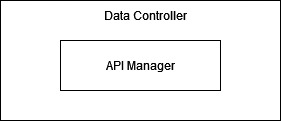
\includegraphics[width=0.60\textwidth]{images/data_controller.jpg}
 \caption{Data controller subsystem diagram}
\end{figure}

\subsubsection{Assumptions}
%Any assumptions made in the definition of the subsystem should be listed and described. Pay particular attention to assumptions concerning interfaces and interactions with other layers.
All of the stores will return grocery descriptions in JSON format. 

\subsubsection{Responsibilities}
%Each of the responsibilities/features/functions/services of the subsystem as identified in the architectural summary must be expanded to more detailed responsibilities. These responsibilities form the basis for the identification of the finer-grained responsibilities of the layer's internal subsystems. Clearly describe what each subsystem does.
The API manager will take a grocery list and give the items in the list to the stores APIs. If the store API will find the given items then it will return the description of the items else it will return an error message. After the API manager gets the data it is responsible for transferring the data to the store manager subsystem. 

\subsubsection{Subsystem Interfaces}
%Each of the inputs and outputs for the subsystem are defined here. Create a table with an entry for each labelled interface that connects to this subsystem. For each entry, describe any incoming and outgoing data elements will pass through this interface.

\begin {table}[H]
\caption {Subsystem interfaces} 
\begin{center}
    \begin{tabular}{ | p{1cm} | p{5cm} | p{3.5cm} | p{3.5cm} |}
    \hline
    ID & Description & Inputs & Outputs \\ \hline
    \#1 & The given grocery is found & \pbox{3cm}{list of grocery items} & \pbox{3cm}{grocery item descriptions}  \\ \hline
    \#2 & The given grocery is not found & \pbox{3cm}{list of grocery items} & \pbox{3cm}{not found message }  \\ \hline
    \end{tabular}
\end{center}
\end{table}

%\subsection{Subsystem 2}
%Repeat for each subsystem

%\subsection{Subsystem 3}
%Repeat for each subsystem

